\documentclass[12pt]{article}
\usepackage{amsmath}
\usepackage{amsfonts}
\usepackage{graphicx}
\usepackage{booktabs}
\usepackage{geometry}
\usepackage[numbers]{natbib}
\geometry{a4paper, margin=1in}
\setlength{\parindent}{0pt}
\setlength{\parskip}{10pt}
\usepackage{float}
\usepackage[labelfont=bf, labelsep=period]{caption}
\captionsetup[figure]{name=Fig.}

\begin{document}
\title{Time Series Analysis for Tesla Stock Prediction Using Machine Learning}

\author{Nguyen Tien Dat-22520226 
\and Vo Quoc Huy-22520***
\and Bui Minh Duy-22520311
\and Cao My Duyen-22520***
\and Nguyen Thien Kim-22520***}
\maketitle



\section{METERIALS}\label{sec:intro}
\subsection{Dataset}
In this study, we scrutinize the historical stock price data for Tesla Inc. (TSLA), sources directly from the Yahoo Finance API. The dataset includes daily information spanning from June 29th, 2010 to May 23th 2025, covering over 3,000 trading days. Each record includes variables that provide important insights and data for the study, specifically as follows:
\begin{itemize}
    \item Date: The specific day the stock price was recorded.
    \item Open: Tesla's stock price at the start of the trading day.
    \item High: The highest price Tesla's stock reached during that day's trading.
    \item Low: The lowest price Tesla's stock dropped to during that day's trading.
    \item Close: Tesla's stock price when the market closed for the day.
    \item Adj Close (Adjusted Close): The closing price, adjusted to account for significant corporate actions like dividends or stock splits.
    \item Volume: The total number of Tesla shares that changed hands on that particular day.
\end{itemize}
To prepare the data for machine learning, we generated several technical indicators from this raw data, including Moving Averages (MA), the Relative Strength Index (RSI), and Moving Average Convergence Divergence (MACD). This data reflects the daily fluctuations in Tesla's stock price and is used to train models that forecast future price trends.
\subsection{Descriptive Statistics}
    

\begin{figure}[H]
    \centering
    \begin{minipage}[b]{0.48\linewidth}
        \centering
        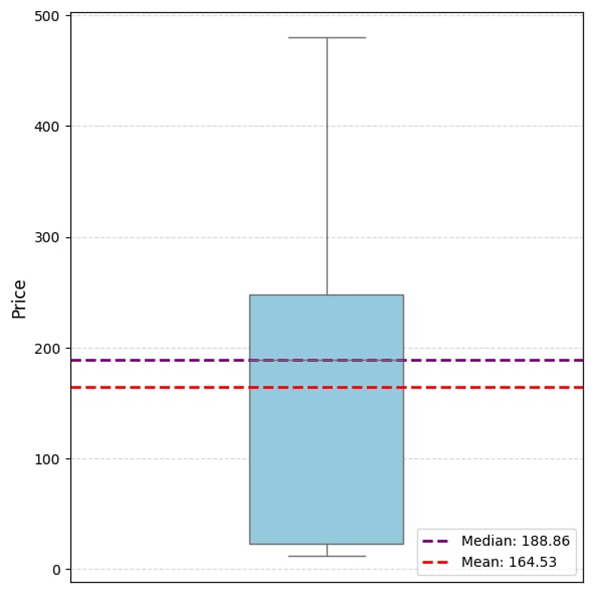
\includegraphics[width=\linewidth]{boxplot.png}
        \caption{TSLA stock price’s boxplot}
        \label{fig:boxplot}
    \end{minipage}
    \hfill
    \begin{minipage}[b]{0.48\linewidth}
        \centering
        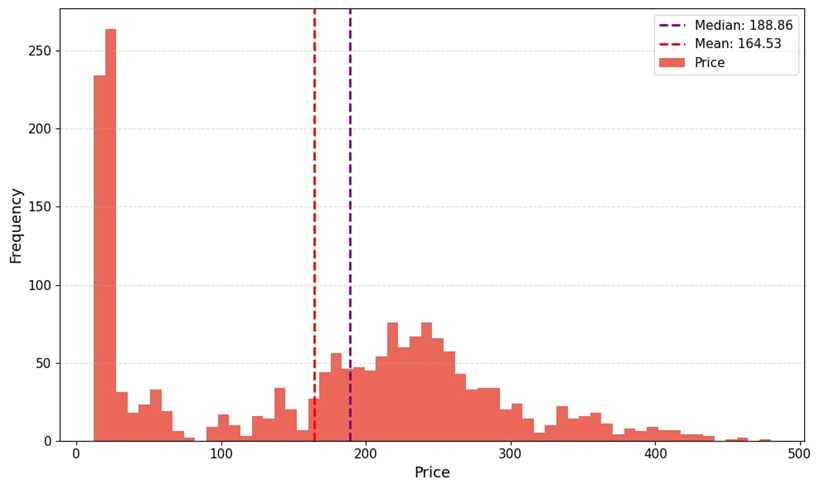
\includegraphics[width=\linewidth]{histogram.png}
        \caption{TSLA stock price’s histogram}
        \label{fig:histogram}
    \end{minipage}
\end{figure}

\begin{table}[H]
    \centering
    \caption{TSLA Descriptive Statistics}
    \label{tab:tsla-stats}
        \begin{tabular}{|c|c|}
        \hline
        \textbf{Descriptive Statistic} & \textbf{TSLA} \\
        \hline
        Count  & 1835 \\
        \hline
        Mean   & 164.525 \\
        \hline
        Std    & 115.339 \\
        \hline
        Min    & 11.931 \\
        \hline
        25\%   & 23.432 \\
        \hline
        50\%   & 188.860 \\
        \hline
        75\%   & 248.197 \\
        \hline
        Max    & 479.860 \\
        \hline
    \end{tabular}
\end{table}

\section{METHODOLOGY}
\subsection{SVR}
SVR extends Support Vector Machines (SVM) to regression tasks. It aims to find a function:
\begin{align}
    f(x) = \langle w, x \rangle + b
\end{align}
that predicts target values within a margin \(\epsilon\) from the true values, while keeping the function as flat as possible \cite{basak2007support}.

\textbf{Primal optimization problem:}
\begin{align}
    \min_{w,b,\xi,\xi^*} \quad \frac{1}{2} \|w\|^2 + C \sum_{i=1}^n (\xi_i + \xi_i^*)
\end{align}
subject to:
\begin{align}
    \begin{cases}
        y_i - \langle w, x_i \rangle - b \leq \epsilon + \xi_i \\
        \langle w, x_i \rangle + b - y_i \leq \epsilon + \xi_i^* \\
        \xi_i, \xi_i^* \geq 0, \quad i=1, \ldots, n
    \end{cases}
\end{align}
\textbf{Where:}
\begin{itemize}
    \item \(\|w\|^2\) controls flatness (regularization).
    \item \(C > 0\) balances model flatness and tolerance for errors greater than \(\epsilon\).
    \item \(\xi_i, \xi_i^*\) are slack variables for deviations outside the \(\epsilon\)-tube.
\end{itemize}
\textbf{Kernel extension (nonlinear SVR):}

By mapping inputs to a higher-dimensional space using a kernel \(K(x_i, x_j) = \phi(x_i)^T \phi(x_j)\), the prediction becomes:

\begin{align}
    f(x) = \sum_{i=1}^n (\alpha_i - \alpha_i^*) K(x_i, x) + b
\end{align}


\subsection{RNN}
A Recurrent Neural Network - RNN is a deep neural network designed to process sequential data such as time series, text, audio,… Unlike traditional feedforward neural networks, RNNs have loops that allow information to persist, making them ideal for tasks where context is crucial.
RNNs process sequential data by maintaining a hidden state that is updated at each time step t, according to the formula \cite{schmidt2019rnn} :
\begin{align}
h^{(t)} &= g_1\left(W_{xh} x^{(t)} + W_{hh} h^{(t-1)} + b_h\right)
\end{align}
With the output being:
\begin{align}
    y^{(t)} &= g_2\left(W_{hy} h^{(t)} + b_y\right)
\end{align}
Where \( y^{\langle t \rangle} \) is the output at time step \( t \), \( W_x \) is the output weight matrix, and \( b_x \) is the output bias term.

\textbf{Where:}
\begin{itemize}
    \item \( x^{(t)} \) is the input vector at time step \( t \).
    \item \( y^{(t)} \) is the output vector at time step \( t \), representing the network's prediction.

    \item \( h^{(t-1)} \) is the hidden state from the previous time step, containing information from prior inputs.
    \item \( W_{xh} \), \( W_{hh} \), and \( W_{hy} \) are weight matrices that transform the inputs and hidden states.
    \item \( b_h \) and \( b_y \) are bias vectors.
    \item \( g_1 \) is a nonlinear activation function (e.g., \(\tanh\) or ReLU) applied to compute the hidden state.
    \item \( g_2 \) is an activation function appropriate for the output task (e.g., softmax for classification).
\end{itemize}




\section{EXPERIMENT}
\subsection{SVR}

\begin{itemize}
    \item \textbf{SVR with Linear Kernel}: \texttt{kernel= linear}, \( C = 100 \)
    \item \textbf{SVR with RBF Kernel}:
    \begin{itemize}
        \item Configuration 1: \( C = 100 \), \( \epsilon = 0.0001 \), \( \gamma = 10 \)
        \item Configuration 2: \( C = 1{,}500{,}000 \), \( \epsilon = 10^{-7} \), \( \gamma = 100 \)
    \end{itemize}
    \item \textbf{SVR with Polynomial Kernel}: \texttt{kernel= poly }, \( C = 100 \), \( \epsilon = 0.0001 \), degree = 3
\end{itemize}
\begin{table}[H]
    \centering
    \caption{RMSE results of SVR models with different kernels}
    \label{tab:svr_results}
    \begin{tabular}{|l|c|}
        \hline
        \multicolumn{1}{|c|}{\textbf{Model}} & \textbf{RMSE} \\
        \hline
        SVR Linear & 0.6342 \\
        SVR RBF (C=100, $\epsilon$=0.0001, $\gamma$=10) & 0.2061 \\
        \textbf{SVR RBF (C=1,500,000, $\epsilon$=1e-7, $\gamma$=100)} & \textbf{0.1306} \\
        SVR Polynomial & 0.7265 \\
        \hline
    \end{tabular}
\end{table}

\begin{figure}[H]
    \centering
    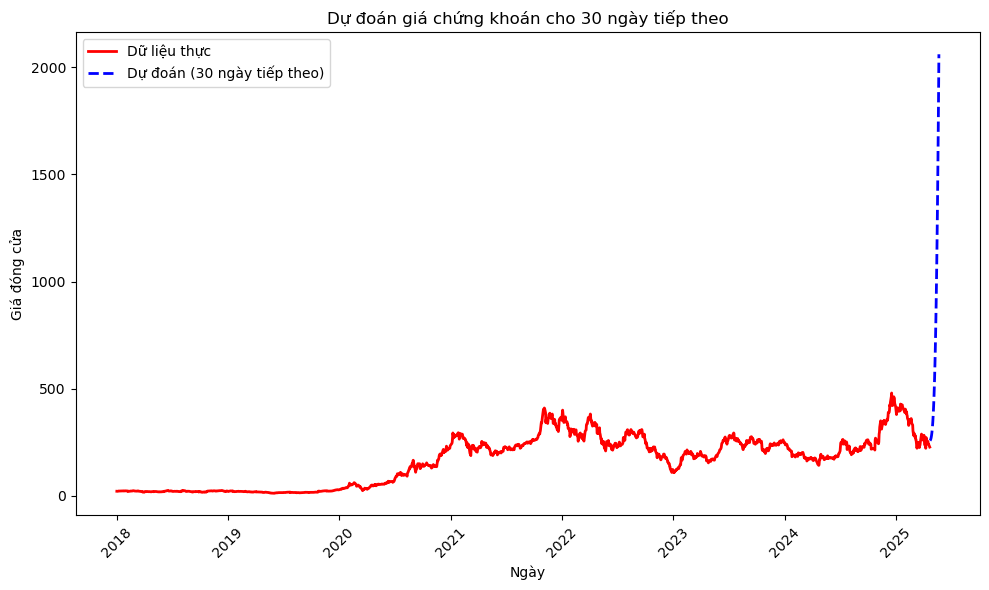
\includegraphics[width=0.5\linewidth]{SVR.png}
    \caption{SVR TSLA 8-2 }
    \label{fig:boxplot}
\end{figure}

\subsection{RNN}

\textbf{Input Layer:} Input shape: $(100, 1)$ — univariate time series with time\_steps $= 100$.

\textbf{SimpleRNN Layer:} 50 units — basic RNN for sequential data processing.

\textbf{Dense Layer (Output Layer):} 1 neuron — linear activation for regression output.

\textbf{Loss function:} Mean Squared Error (MSE) — suitable for regression tasks.

\textbf{Optimizer:} Adam — adaptive learning rate.

\textbf{Epochs:} 24 — full passes over the training data.

\textbf{Batch size:} 64 — samples per gradient update.

\textbf{Verbose:} 1 — show training progress.

\begin{figure}[H]
    \centering
    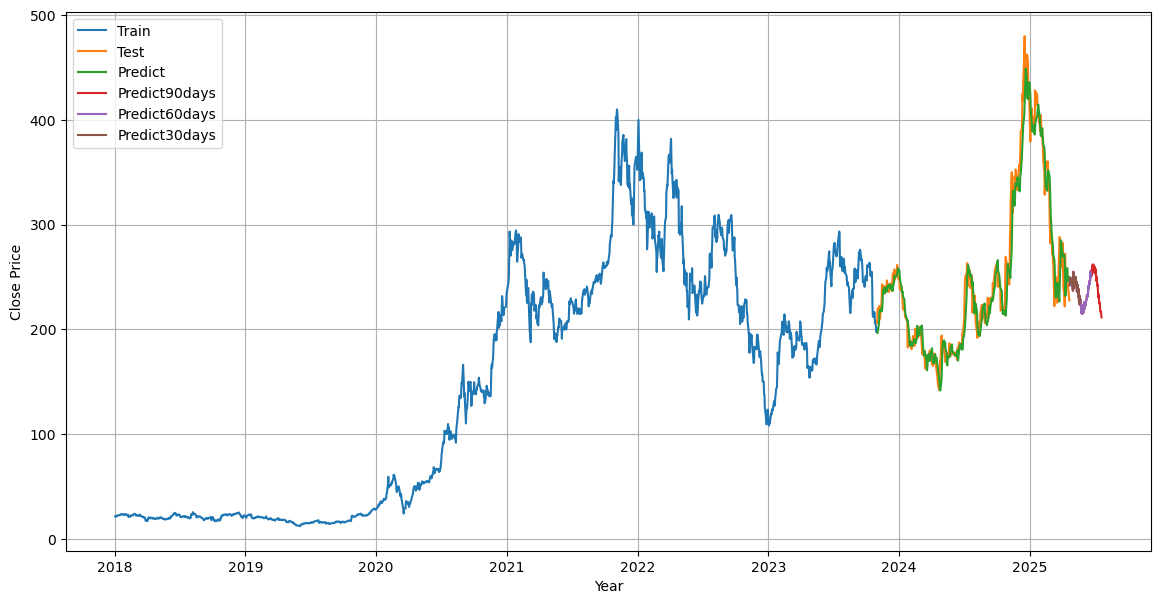
\includegraphics[width=0.5\linewidth]{RNN.png}
    \caption{RNN TSLA 8-2 }
    \label{fig:boxplot}
\end{figure}



\renewcommand{\refname}{References}
\bibliographystyle{plainnat}  % hoặc unsrtnat nếu bạn muốn theo thứ tự xuất hiện

\bibliography{references} % Link to references.bib
\end{document}